\documentclass[a4paper,12pt,titlepage]{article}

% Paquetes para soporte de idioma y codificación

\usepackage{lmodern}
\usepackage[spanish,es-tabla]{babel}

% Paquetes para representar símbolos matemáticos
\usepackage{amsmath}
\usepackage{amssymb}
\usepackage{amsfonts}
\usepackage{amsthm}
\usepackage{mathtools}

% Paquetes gráficos y de diagramas
\usepackage{tikz}
\usetikzlibrary{shapes, arrows, arrows.meta, positioning, calc}
% Configuración de estilos corregida
\tikzset{
    startstop/.style={draw, rectangle, rounded corners, minimum width=3cm, minimum height=1cm, text centered, align=center, line width=1pt, fill=blue!10},
    process/.style={draw, rectangle, minimum width=3.5cm, minimum height=1cm, text centered, align=center, fill=orange!10},
    decision/.style={draw, diamond, aspect=1.5, minimum width=3.5cm, minimum height=1cm, text centered, align=center, fill=green!10},
    arrow/.style={thick, ->, >=Stealth}
}
\usepackage{graphicx}
\usepackage{float}
\usepackage{pgfplots}
\pgfplotsset{compat=1.18}

% Paquete para listados de código fuente
\usepackage{listings}
\usepackage{xcolor}

% Configuración estética para los fragmentos de código Java/pseudocódigo
\definecolor{codegreen}{rgb}{0,0.6,0}
\definecolor{codegray}{rgb}{0.5,0.5,0.5}
\definecolor{codepurple}{rgb}{0.58,0,0.82}
\definecolor{backcolour}{rgb}{0.96,0.96,0.94}

\lstset{
    backgroundcolor=\color{backcolour},   
    commentstyle=\color{codegreen},
    keywordstyle=\color{blue}\bfseries,
    numberstyle=\tiny\color{codegray},
    stringstyle=\color{codepurple},
    basicstyle=\ttfamily\small,
    breakatwhitespace=false,         
    breaklines=true,                 
    captionpos=b,                    
    keepspaces=true,                 
    numbers=left,                    
    numbersep=5pt,                  
    showspaces=false,                
    showstringspaces=false,
    showtabs=false,                  
    tabsize=4,
    frame=single,
    rulecolor=\color{gray!30}
}

% Paquetes de formato de página y tablas
\usepackage{booktabs}
\usepackage{geometry}
\geometry{left=3cm,right=2cm,top=2cm,bottom=2cm}
\usepackage{hyperref}
\hypersetup{
    colorlinks=true,
    linkcolor=blue,
    filecolor=magenta,      
    urlcolor=cyan,
    pdftitle={Análisis de seguridad e implementación algorítmica de GOST R 34.10},
    pdfpagemode=FullScreen,
}

% Definición de entornos matemáticos estructurados
\newtheorem{theorem}{Teorema}[section]
\newtheorem{definition}{Definición}[section]
\newtheorem{property}{Propiedad}[section]

\begin{document}

% --- PORTADA ---
\begin{titlepage}
    \centering
    \vspace*{2cm}
    {\Huge\bfseries Análisis de seguridad e implementación algorítmica del estándar criptográfico ruso de firmas digitales GOST R 34.10\par}
    
    \vspace{3.5cm}
{\Large\bfseries Integrantes:\par}
\vspace{0.5cm}
{\large 
\begin{tabular}{l @{\hspace{1.5cm}} l}
    Aldo Luna Bueno & 20170325B \\
    Joel Benjamín Seminario Serna & 20210056G \\
    Jharvy Jonas Cadillo Tarazona & 20210184E \\
    Melissa Iman Noriega & 20224041G \\
    Luis Alberto Alanya Campos & 20210290J
    
\end{tabular}\par}
    
    \vspace{3.5cm}
    {\Large Universidad Nacional de Ingeniería\par}
    \vspace{0.2cm}
    {\large Escuela Profesional de Ciencia de la Computación\par}
    \vfill
    {\large \today \par}
\end{titlepage}

\section{Introducción}

\subsection{Contexto y motivación}
La firma digital asegura tres principios: la integridad del mensaje, la autenticidad del emisor y el no repudio. Algoritmos como RSA dominaron este campo en el pasado, pero la Criptografía de Curvas Elípticas es el estándar moderno debido a su capacidad de ofrecer niveles de seguridad equivalentes con tamaños de clave drásticamente menores, lo que optimiza el rendimiento computacional y el ancho de banda.

Las naciones y bloques han desarrollado sus propios estándares para garantizar la soberanía de sus comunicaciones. Mientras que Occidente ha estandarizado mayoritariamente ECDSA (del instituto NIST), la Federación Rusa emplea el estándar GOST R 34.10-2012. El estudio e implementación de estándares alternativos no solo amplía la perspectiva técnica sobre las decisiones de diseño criptográfico, sino que permite comprender las sutilezas matemáticas de las curvas de Weierstrass bajo diferentes dominios de parámetros.

Al adoptar una metodología de Desarrollo Guiado por Pruebas (TDD) y una arquitectura modular orientada a interfaces en Java, este trabajo busca demostrar que las matemáticas abstractas de los cuerpos finitos pueden traducirse en sistemas de software robustos, verificables y resistentes a vulnerabilidades de implementación.

\subsection{Objetivos del proyecto}

\textbf{Objetivo General:} \\
Analizar, diseñar e implementar desde cero el estándar de firma digital electrónica GOST R 34.10-2012, junto con su función hash criptográfica asociada GOST R 34.11-2012 (Streebog), garantizando la exactitud matemática y la seguridad algorítmica mediante pruebas unitarias rigurosas.

\vspace{0.3cm}
\noindent\textbf{Objetivos Específicos:}
\begin{itemize}
    \item \textbf{Modelamiento Matemático:} Desarrollar un motor algebraico seguro para operaciones sobre curvas elípticas en el cuerpo finito $\mathbb{F}_p$, implementando la suma de puntos, duplicación y multiplicación escalar (Double-and-Add), con mitigaciones integradas contra ataques de curva inválida.
    \item \textbf{Implementación de Función Hash:} Codificar el algoritmo de compresión criptográfica Streebog, asegurando el correcto procesamiento de la memoria bajo restricciones Little-Endian y el cumplimiento de las reglas modulares del estándar.
    \item \textbf{Desarrollo del Protocolo de Firma:} Construir de manera desacoplada los módulos del Emisor (Algoritmo I - Generación de firma) y del Receptor (Algoritmo II - Verificación de firma), manejando correctamente los inversos modulares y la entropía criptográfica ($k$).
    \item \textbf{Validación y Calidad de Software:} Comprobar la exactitud de cada componente mediante la automatización de pruebas unitarias (JUnit) inyectando los vectores de control estandarizados en los apéndices oficiales (RFC 6986 y GOST).
    \item \textbf{Evaluación de Seguridad:} Analizar las vulnerabilidades inherentes a una mala implementación del estándar y establecer un marco comparativo a nivel arquitectónico y de seguridad entre GOST R 34.10 y ECDSA.
\end{itemize}

\subsection{Organización del documento}
El presente informe está estructurado para guiar al lector desde los fundamentos teóricos hasta la ejecución y análisis del código fuente. En el Capítulo 2, se expone el marco teórico, abarcando la matemática de las curvas elípticas sobre cuerpos finitos y los conceptos de firma digital. El Capítulo 3 detalla la justificación metodológica, explicando la arquitectura del sistema, la separación de responsabilidades a través de interfaces y el enfoque TDD.

En el Capítulo 4, se documenta el núcleo del trabajo: la implementación algorítmica detallada de la función Hash Streebog, y los procesos de generación y verificación de la firma. El Capítulo 5 profundiza en la ciberseguridad, analizando las estrategias de mitigación de ataques programadas en el código y ofreciendo una comparativa analítica frente a otros estándares globales. Finalmente, el Capítulo 6 expone las conclusiones del proyecto, seguido de las referencias bibliográficas y los anexos que contienen el código fuente fundamental.
\section{Fundamentos Teóricos}

\subsection{¿Qué es una curva elíptica?}

La criptografía en general nos ha acostumbrado a pensar que la seguridad se debe basar en un simple juego aritmético, pero este estándar de las curvas elípticas nos muestra que también podemos hacer criptografía con geometría. 

Una curva elíptica es un conjunto de puntos que satisfacen la ecuación en forma normal de Weierstrass $y^2 = x^3 + ax + b$ cuyo discriminante $4a^3 + 27b^2$ debe ser distinto de cero para evitar singularidades (curvas con auto-intersecciones o cúspides) e incluye además un elemento teórico indispensable llamado punto en el infinito (denotado como $0$).

\begin{definition} Curva elíptica. $$\left\{ (x, y) \in \mathbb{R}^2 \mid y^2 = x^3 + ax + b, \ 4a^3 + 27b^2 \neq 0 \right\} \cup \{0\}$$
\end{definition}

Pero si no hay una operación, no podemos hacer nada con la curva o con sus puntos. Por eso definimos la operación de suma así:

\begin{definition}
\textbf{Si trazamos una línea recta y cruza tres puntos de la curva ($P$, $Q$ y $R$), su suma es cero ($P + Q + R = 0$).}
\end{definition}

Esta definición geométrica de suma tiene la bondad de que convierte a los puntos de la curva en un grupo abeliano, con lo cual emergen muchas propiedades útiles, como la unicidad del elemento neutro o del elemento inverso aditivo. Pero nuestra definición es ternaria. Necesitamos hacerla más operativa.

Para sumar $P + Q$, se traza una línea entre ambos, se encuentra el tercer punto de intersección $R$ en la curva y se toma su reflejo sobre el eje X (es decir, $-R$). Por lo tanto, $P + Q = -R$. 

\begin{figure}[H]
    \centering
    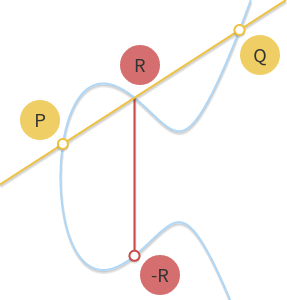
\includegraphics[width=0.5\textwidth]{imagenes/suma_cuerpo_reales.png}
    \caption{Operación geométrica de la suma  $P + Q = -R$, con puntos $P$, $Q$ y $R$ colineales en una curva elíptica sobre los reales.}
    \label{fig:suma_cuerpo_reales}
\end{figure}

Al pasar esto al álgebra, la suma requiere calcular la pendiente de la recta ($m$) entre los puntos para encontrar las coordenadas exactas del nuevo punto.

Si $P$ y $Q$ son distintos ($x_P \neq x_Q$), la línea tiene pendiente:

$$m = \frac{y_P - y_Q}{x_P - x_Q}$$


Si, por el contrario, $P$ y $Q$ son iguales, la pendiente se debe calcular de otra manera. La línea se ve como una tangente a la curva en este punto. Si queremos calcular la pendiente de una tangente, derivamos la ecuación de la curva en ese punto. Nos queda la siguiente expresión:

$$m = \frac{3x_P^2 + a}{2y_P}$$

En cualqueir caso, la intersección entre la línea y esta curva es un tercer punto: $R = (x_R, y_R)$:

$$
\begin{aligned}
x_R &= m^2 - x_P - x_Q \\
y_R &= y_P + m(x_R - x_P) = y_Q + m(x_R - x_Q)
\end{aligned}
$$

De esta manera, $(x_P, y_P) + (x_Q, y_Q) = (x_R, -y_R)$ (recordemos $P + Q = -R$).

\subsection{¿Podemos hacer criptografía con estas curvas elípticas?}

La respuesta corta: \textbf{no}. Más adelante veremos que necesitamos efectuar la operación de suma cientos de veces iterativamente. Si bien sobre el papel tienen propiedades muy intersantes, si trabajamos sobre el cuerpo de los números reales, el error propagado sobre puntos de la curva calculados se haría enorme y no sería un método confiable. 

Para usar las curvas en criptografía, debemos abandonar el conjunto de los números reales y definir la curva elíptica sobre un cuerpo finito de enteros módulo un número primo.

\begin{definition} Curva elíptica sobre cuerpo finito $\mathbb{F}_p$.
$$\{ (x, y) \in (\mathbb{F}_p)^2 \mid y^2 \equiv x^3 + ax + b \pmod p, 4a^3 + 27b^2 \not\equiv 0 \pmod p \} \cup \{0\}$$
\end{definition}

Esto tiene varias consecuencias:
\begin{itemize}
    \item La curva se vuelve un conjunto de puntos discretos representados por $y^2 \equiv x^3 + ax + b \pmod{p}$.
    \item Es necesario redefinir qué entendemos por puntos colineales.
    \item Las ecuaciones algebraicas para sumar puntos siguen siendo exactamente las mismas, pero todas las operaciones aritméticas (suma, resta, multiplicación) se calculan con el módulo $p$.
    \item La ``división'' en un cuerpo finito requiere encontrar el inverso multiplicativo mediante el algoritmo de Euclides extendido.
\end{itemize}

Es importante notar una propiedad fundamental de la aritmética modular en este paso: la operación de ``división'' (es decir, multiplicar por el inverso multiplicativo $(x_P - x_Q)^{-1} \bmod p$) solo está matemáticamente definida si el denominador $(x_P - x_Q)$ y el módulo $p$ son coprimos. Dado que en la criptografía de curvas elípticas $p$ se elige siempre como un número primo, esta condición de coprimalidad está garantizada para cualquier diferencia temporal, salvo cuando el denominador se anula por completo (es decir, cuando $x_P = x_Q$). Es en ese escenario exacto donde la fórmula de la recta secante deja de ser válida y el álgebra nos obliga, de forma natural, a transicionar a la fórmula de la pendiente de la recta tangente.

\begin{figure}[H]
    \centering
    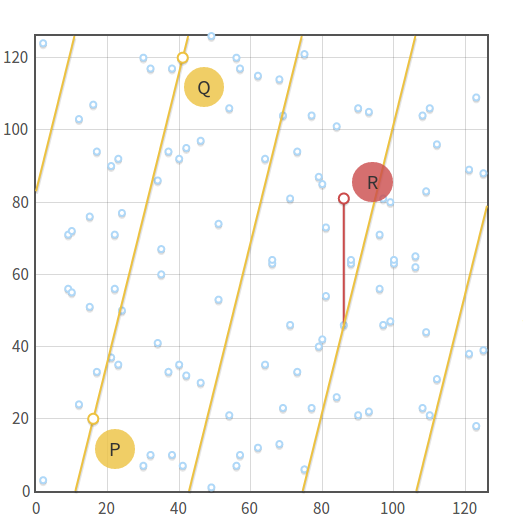
\includegraphics[width=0.5\textwidth]{imagenes/suma_cuerpo_finito.png}
    \caption[Suma de puntos sobre la curva en cuerpo finito]{Suma de puntos sobre la curva $y^2 \equiv x^3 - x + 3 \pmod{127}$, con $P = (16, 20)$ y $Q = (41, 120)$. Nótese que la línea $y \equiv 4x + 83 \pmod{127}$ que conecta los puntos se repite en el plano.}
    \label{fig:suma_cuerpo_finito}
\end{figure}

Entonces, dados los puntos colineales $P = (x_P, y_P)$, $Q = (x_Q, y_Q)$ y $R = (x_R, y_R)$, calculamos $P + Q = -R$ así:

Si $P \neq Q$, la pendiente $m$ se calcula como:

$$m = (y_P - y_Q)(x_P - x_Q)^{-1} \bmod p$$

De lo contrario, si $P = Q$, la pendiente se calcula así:

$$m = (3x_P^2 + a)(2y_P)^{-1} \bmod p$$

Y usamos este resultado en las nuevas expresiones modulares:

$$\begin{aligned}
x_R &= (m^2 - x_P - x_Q) \bmod p \\
y_R &= [y_P + m(x_R - x_P)] \bmod p \\
&= [y_Q + m(x_R - x_Q)] \bmod p
\end{aligned}$$

Y es así que finalmente calculamos:

$$P + Q = -R = (x_R, -y_R \bmod p)$$

\subsection{¿Hay algún orden en este aparente caos?}

Si sumamos puntos en $\mathbb{F}_p$, los resultados saltan por todo el plano de forma aparentemente caótica. ¿Cómo confiamos en algo caótico?

Saber que una curva elíptica sobre un cuerpo finito $\mathbb{F}_p$ forma un grupo abeliano bajo la operación de suma de puntos no es suficiente para garantizar la viabilidad de un protocolo; necesitamos conocer la topología exacta de este grupo, denotado como $E(\mathbb{F}_p)$. Es aquí donde interviene una pieza clave del álgebra abstracta.

\begin{theorem} Teorema Fundamental de los Grupos Abelianos Finitos.
Todo grupo abeliano finito es isomorfo a un producto directo de grupos cíclicos cuyos órdenes son potencias de números primos.
\end{theorem}

Al aplicar este teorema a la teoría de curvas algebraicas, obtenemos un resultado maravillosamente restrictivo y preciso. Nos garantiza que el grupo de puntos $E(\mathbb{F}_p)$ es isomorfo a, como máximo, el producto de dos grupos cíclicos:

$$E(\mathbb{F}_p) \cong \mathbb{Z}_{q_1} \times \mathbb{Z}_{q_2}$$

Donde $q_1$ y $q_2$ son enteros positivos tales que $q_1$ divide a $q_2$, y a su vez $q_1$ divide a $p-1$. En el caso particular (y muy buscado en criptografía) donde $q_1 = 1$, la curva forma un único grupo cíclico $\mathbb{Z}_{q_2}$.

Saber que la curva se descompone matemáticamente en esta estructura fundamenta la aplicación de estándares como el GOST R 34.10 en tres aspectos críticos:

\begin{itemize}
    \item \textbf{Selección del punto generador ($P$):} Para hacer criptografía, requerimos un punto base $P$ que, al someterse a multiplicación escalar sucesiva, genere una trayectoria predecible y extensa antes de alcanzar el punto en el infinito ($0$). El teorema nos asegura la existencia de un generador para un subgrupo cíclico de orden estricto $q$.
    \item \textbf{Base del Logaritmo Discreto:} La seguridad de los protocolos de firma digital no opera sobre la totalidad de los puntos de la curva, sino confinada dentro de un subgrupo cíclico principal. El teorema garantiza matemáticamente la existencia y la delimitación de estos subgrupos.
    \item \textbf{Evasión de vulnerabilidades:} Conocer la descomposición en $\mathbb{Z}_{q_1} \times \mathbb{Z}_{q_2}$ permite auditar la curva. Si el orden del subgrupo cíclico ($q$) se llegara a factorizar en números primos pequeños, algoritmos como el de Pohlig-Hellman podrían quebrar la clave reduciendo el problema a subgrupos menores. Gracias a esta certeza algebraica, los criptógrafos configuran los parámetros para asegurar que el orden $q$ sea un primo inmenso, neutralizando este vector de ataque.
\end{itemize}

\subsection{¿Cómo aplicamos las curvas elípticas a la criptografía?}

Si sumamos un punto $P$ consigo mismo $n$ veces ($nP = P + P + \dots + P$), obtenemos un nuevo punto de la curva. Esta operación llamada multiplicación escalar es la base directa de la criptografía de curva elíptica.

\begin{definition} Multiplicación escalar.
$$nP = \underbrace{P + P + \dots + P}_{n \text{ veces}}$$
\end{definition}

En una aplicación criptográfica seria vamos a tener un escalar $n$ de cientos de cifras. Para un escalar $n$ de $k$ bits, que es como realmente se miden estos números en criptografía, el algoritmo de sumar de uno en uno los puntos $P$ tiene una complejidad temporal $\mathcal{O}(2^k)$, inalcanzable computacionalmente. Para esto se diseñó el algoritmo de ``doblar y sumar'' (\textit{double and add}), el cual descompone $n$ en potencias de dos a partir de su representación binaria. Esto reduce drásticamente el tiempo de cómputo a una complejidad de $\mathcal{O}(k)$, volviendo la operación fácil y rápida para las computadoras.


\begin{figure}[H]
    \centering
    \begin{tikzpicture}[node distance=0.8cm and 2cm]

        % Bloques principales
        \node (start) [startstop] {Inicio \\ \small (Entrada: $n, P$)};
        
        \node (init) [process, below=of start] {\texttt{result} = 0 \\ \texttt{addend} = $P$};
        
        \node (while_cond) [decision, below=of init] {¿Quedan bits \\ en $n$?};
        
        % Eliminamos el \& problemático usando \texttt
        \node (get_bit) [process, below=of while_cond] {\texttt{bit} = \texttt{least\_significant\_bit(n)} \\ n = \texttt{right\_shift(n)}};
        
        \node (check_bit) [decision, below=of get_bit] {¿\texttt{bit} == 1?};
        
        \node (add_step) [process, below=of check_bit] {\texttt{result} += \texttt{addend}};
        
        \node (double_step) [process, below=1.2cm of add_step] {\texttt{addend} *= 2};
        
        \node (stop) [startstop, right=of while_cond] {Fin \\ \small (Retorna \texttt{result})};

        % Conexiones y flujos
        \draw [arrow] (start) -- (init);
        \draw [arrow] (init) -- (while_cond);
        
        % De la condición del bucle (While)
        \draw [arrow] (while_cond) -- node[anchor=east] {Sí} (get_bit);
        \draw [arrow] (while_cond) -- node[anchor=south] {No} (stop);
        
        \draw [arrow] (get_bit) -- (check_bit);
        
        % Condicional del bit (If bit == 1)
        \draw [arrow] (check_bit) -- node[anchor=east] {Sí} (add_step);
        \draw [arrow] (add_step) -- (double_step);
        
        % Camino "No" del condicional del bit
        \draw [arrow] (check_bit.west) -- node[anchor=south] {No} ++(-1.5cm,0) |- (double_step.west);
        
        % Retroalimentación del bucle (Regresar a evaluar la condición)
        \draw [arrow] (double_step.east) -- ++(2cm,0) |- (while_cond.south east);

    \end{tikzpicture}
    \caption{Diagrama de flujo del algoritmo \textit{Double and Add}.}
    \label{fig:double_and_add}
\end{figure}

Al multiplicar un punto base $P$ repetidas veces sobre un cuerpo finito, los resultados no cubren toda la curva, sino que forman un subgrupo cíclico que se repite infinitamente (por ejemplo: $P, 2P, 3P, 4P, 0$).
\begin{itemize}
    \item \textbf{Orden del subgrupo ($n$):} Es la cantidad de puntos que tiene el ciclo y equivale al menor número $n$ para el cual $nP = 0$.
    \item \textbf{Teorema de Lagrange:} Establece que el orden de este subgrupo ($n$) siempre debe ser un divisor exacto del orden total de puntos que tiene la curva elíptica completa ($N$).
    \item \textbf{Cofactor ($h$):} Es el resultado de dividir el orden total de la curva entre el orden del subgrupo ($h = N / n$). En criptografía, se busca que $n$ sea un número primo muy grande y se usa el cofactor para encontrar un punto generador ($G$) seguro multiplicando un punto aleatorio $P$ por $h$ ($G = hP$).
\end{itemize}

Si bien calcular la múltiplicación escalar para un $n$ elevado es fácil, el problema inverso de encontrar $n$ sabiendo $P$ y $nP$ es extremadamente difícil. Este es llamado el Problema del Logaritmo Discreto (DLP), y es el corazón de la seguridad del sistema. 

\begin{definition} Problema del Logaritmo Discreto (DLP).
Si conocemos un punto base $P$ y otro punto $Q$ en una curva elíptica sobre $\mathbb{F}_p$, ¿cuál es el número $n$ tal que $Q = nP$? \\
\end{definition}

Debido a que la multiplicación escalar sobre cuerpos finitos parece caótica y da saltos discretos impredecibles en el plano, resolver este Problema del logaritmo discreto es computacionalmente ``difícil''. No existe ningún algoritmo de tiempo polinómico para computadoras clásicas que pueda encontrar el número secreto $n$ fácilmente. Esta asimetría matemática (fácil de multiplicar, inviable de revertir) es lo que garantiza que la clave privada permanezca segura.

El estándar criptográfico ruso GOST R 34.10-2012 se apoya exactamente en esta fundamentación matemática, operando sobre curvas elípticas en forma de Weierstrass con cuerpos finitos primos de $256$ o $512$ bits. Los parámetros de la curva (como $a$, $b$, el primo $p$ y el generador $P$) están estrictamente definidos por el estándar para garantizar que el cofactor $h$ sea óptimo y evite subgrupos débiles.
\section{Metodología de Desarrollo e Integración}

El desarrollo de software criptográfico impone requisitos críticos de exactitud matemática y seguridad en la gestión de memoria. Un mínimo error en la manipulación de bits o en la aritmética modular puede resultar en vulnerabilidades catastróficas. Por ello, este proyecto descartó el desarrollo empírico tradicional en favor de una metodología orientada a la verificación continua y la segregación arquitectónica.

\subsection{Arquitectura Orientada a Interfaces}
Para permitir el desarrollo en paralelo y mitigar los bloqueos entre los miembros del equipo, el sistema se diseñó bajo el principio de Segregación de Interfaces (SOLID). Se definieron contratos estrictos (\textit{interfaces} en Java) para los tres componentes principales del estándar: el módulo de \textit{hashing} criptográfico (\texttt{HashService}), la generación de firmas (\texttt{SignatureGenerator}) y la verificación de firmas (\texttt{SignatureVerifier}). 

Esta abstracción garantizó que cada módulo interactuara con los demás únicamente a través de tipos de datos puros y Objetos de Transferencia de Datos (DTOs), eliminando dependencias circulares y facilitando el aislamiento necesario para las pruebas de calidad.

\subsection{Desarrollo Guiado por Pruebas (TDD) con JUnit 5}
La piedra angular de la metodología del proyecto fue la adopción estricta del Desarrollo Guiado por Pruebas (TDD, por sus siglas en inglés). En lugar de programar la lógica del estándar y probarla al final, se codificaron primero las pruebas unitarias utilizando el marco de trabajo JUnit 5. 

El marco de aserción se construyó extrayendo los vectores de prueba oficiales (entradas estáticas y sus salidas matemáticas esperadas) publicados en los apéndices de los documentos GOST R 34.10-2012 y RFC 6986. De esta forma, el código de implementación se consideraba completo única y exclusivamente cuando lograba satisfacer las aserciones estandarizadas.

Para asegurar la legibilidad y mantenibilidad del conjunto de pruebas, cada test unitario se estructuró siguiendo el patrón \textbf{AAA (Arrange, Act, Assert)}:
\begin{itemize}
    \item \textbf{Arrange (Preparar):} Se inicializan los objetos, se configuran las dependencias y se declaran las constantes estáticas (vectores de prueba) extraídas del estándar.
    \item \textbf{Act (Ejecutar):} Se invoca el método principal del componente criptográfico.
    \item \textbf{Assert (Afirmar):} Se evalúa si el resultado de la ejecución coincide exactamente con el vector de control.
\end{itemize}

El siguiente fragmento de código ilustra la aplicación del patrón AAA en la validación del flujo completo del Emisor (Algoritmo I). Para lograr una prueba determinista y replicable, se utilizó una sobrecarga del método que permite inyectar el número aleatorio efímero ($k$), evaluando así el ``camino feliz'' contra los valores exactos del Apéndice A.1:

\begin{lstlisting}[language=Java, caption={Prueba unitaria del Emisor estructurada bajo el patrón AAA (cadenas hexadecimales truncadas por brevedad)}, label={lst:aaa_pattern}]
@Test
public void testSignWithAppendixA1Vectors() {
    // 1. Arrange (Preparar)
    // Configuracion de parametros de dominio (256 bits)
    BigInteger p = new BigInteger("80000000...0431", 16);
    BigInteger a = new BigInteger("7", 16);
    BigInteger b = new BigInteger("5FBFF498...3B7E", 16);
    BigInteger q = new BigInteger("80000000...F5B3", 16);
    Point P = new Point(
        new BigInteger("2", 16),
        new BigInteger("8E2A8A0E...E8FC8", 16)
    );
    DomainParameters params = new DomainParameters(p, a, b, q, P);

    // Entradas estaticas del documento oficial
    BigInteger e = new BigInteger("2DFBC1B3...3EE5", 16); // Hash
    BigInteger d = new BigInteger("7A929ADE...3B28", 16); // Clave privada
    BigInteger k = new BigInteger("77105C9B...EAB3", 16); // Nonce determinista

    // Valores esperados de la firma
    BigInteger expectedR = new BigInteger("41AA28D2...0493", 16);
    BigInteger expectedS = new BigInteger("1456C64B...9C40", 16);

    // 2. Act (Ejecutar)
    Signature firma = signer.sign(e, d, k, params);

    // 3. Assert (Afirmar)
    assertEquals(expectedR, firma.r, "Fallo en R (C = kP)");
    assertEquals(expectedS, firma.s, "Fallo en S (s = (rd + ke) mod q)");
}
\end{lstlisting}

Este enfoque de pruebas permitió validar la exactitud de las implementaciones abstractas, asegurando que cualquier desviación en el cálculo modular o en la multiplicación escalar sobre la curva elíptica fuese detectada de manera inmediata antes de la fase de integración final.

\subsection{Gestión de la Precisión Arbitraria y Convenciones de Memoria}
El estándar GOST exige realizar operaciones algebraicas sobre cuerpos finitos utilizando números de 256 y 512 bits. Dado que los tipos de datos primitivos de Java (como \texttt{long}) están limitados a 64 bits, la arquitectura base se cimentó íntegramente sobre la clase nativa \texttt{java.math.BigInteger}. Esta decisión eliminó el riesgo de desbordamientos aritméticos (\textit{overflows}) y proporcionó rutinas optimizadas para operaciones fundamentales como la multiplicación modular y el cálculo de inversos multiplicativos.

Adicionalmente, se desarrolló una utilidad centralizada (\texttt{GostUtils}) para gobernar el ordenamiento de bytes. Puesto que los estándares criptográficos rusos imponen el formato \textit{Little-Endian} para la representación de vectores en memoria, mientras que la Máquina Virtual de Java (JVM) opera por defecto en \textit{Big-Endian}, esta abstracción centralizada previno inconsistencias sistémicas durante el intercambio de datos entre la función Hash, el Emisor y el Receptor.

\subsection{Gestión de la Precisión Arbitraria y Convenciones de Memoria}
El estándar GOST exige realizar operaciones algebraicas sobre cuerpos finitos utilizando números de 256 y 512 bits. Dado que los tipos de datos primitivos de Java (como \texttt{long}) están limitados a 64 bits, la arquitectura base se cimentó íntegramente sobre la clase nativa \texttt{java.math.BigInteger}. Esta decisión eliminó el riesgo de desbordamientos aritméticos (\textit{overflows}) y proporcionó rutinas optimizadas para operaciones fundamentales como la multiplicación modular y el cálculo de inversos multiplicativos.

Adicionalmente, se desarrolló una utilidad centralizada (\texttt{GostUtils}) para gobernar el ordenamiento de bytes. Puesto que los estándares criptográficos rusos imponen el formato \textit{Little-Endian} para la representación de vectores en memoria, mientras que la Máquina Virtual de Java (JVM) opera por defecto en \textit{Big-Endian}, esta abstracción centralizada previno inconsistencias sistémicas durante el intercambio de datos entre la función Hash, el Emisor y el Receptor.
\section{Implementación algorítmica}

En esta sección se detalla el diseño e implementación del sistema criptográfico, abordando desde la construcción del motor de compresión (Streebog) hasta los protocolos de generación y verificación distribuidos en módulos independientes.

\subsection{Módulo de Compresión Criptográfica (Streebog)}

La primera etapa del proceso de firma digital consiste en transformar el mensaje original en un resumen criptográfico de longitud fija. Para ello se implementó el algoritmo Streebog, definido por el estándar ruso GOST R 34.11-2012, cuya función principal es producir una representación compacta del mensaje preservando las propiedades fundamentales de integridad, resistencia a colisiones y resistencia a ataques de preimagen.

Dentro de la arquitectura desarrollada, el módulo Streebog actúa como punto de entrada del flujo criptográfico. Antes de que el algoritmo de firma pueda operar sobre el mensaje, este debe ser procesado por la función hash para obtener un valor numérico de tamaño controlado. Esta estrategia evita que el algoritmo de firma trabaje directamente sobre mensajes de longitud arbitraria y permite que todo el procesamiento posterior se realice sobre estructuras matemáticas compatibles con los grupos definidos por la curva elíptica.

La implementación fue diseñada para soportar las dos variantes oficiales del estándar: Streebog-256 y Streebog-512. Ambas versiones comparten la misma estructura interna de compresión, diferenciándose únicamente en el tamaño del resumen producido. La selección de la variante se realiza mediante un parámetro configurable durante la creación de la instancia del servicio de hashing.

Una de las consideraciones más importantes durante el desarrollo fue el manejo correcto del ordenamiento de bytes. A diferencia de muchos estándares occidentales que emplean representaciones Big-Endian, los estándares criptográficos rusos utilizan de forma predominante la representación Little-Endian. Esta diferencia puede generar errores sutiles durante la conversión de datos binarios a enteros arbitrariamente grandes. Para evitar inconsistencias se desarrolló una utilidad centralizada encargada de realizar las transformaciones de endianness requeridas por el estándar.

Una vez obtenido el resumen criptográfico, el estándar GOST R 34.10 exige convertir dicho valor a un entero positivo denominado $e$. Este entero será posteriormente utilizado durante la generación y verificación de firmas digitales. El procedimiento consta de tres etapas:

\begin{enumerate}
    \item Interpretar el hash como un entero positivo utilizando la convención Little-Endian.
    \item Aplicar una reducción módulo $q$, donde $q$ representa el orden del subgrupo criptográfico utilizado por la curva elíptica.
    \item Aplicar la regla especial del estándar que establece que si el resultado es cero, entonces debe reemplazarse por el valor uno.
\end{enumerate}

Matemáticamente:

\[
\alpha = \text{LittleEndianToInteger}(Hash)
\]

\[
e = \alpha \bmod q
\]

y si

\[
e = 0
\]

entonces

\[
e = 1
\]

La implementación desarrollada para este procedimiento se muestra a continuación.

\begin{lstlisting}[language=Java, caption={Conversión del hash Streebog al entero utilizado por GOST.}]
public BigInteger formatToGostInteger(byte[] rawHashBytes,
                                      BigInteger q) {

    BigInteger alpha =
        GostUtils.fromLittleEndianBytes(rawHashBytes);

    BigInteger e = alpha.mod(q);

    if (e.equals(BigInteger.ZERO)) {
        e = BigInteger.ONE;
    }

    return e;
}
\end{lstlisting}

Con el objetivo de garantizar la exactitud de la implementación se desarrolló una batería de pruebas unitarias utilizando JUnit 5. Las pruebas fueron construidas siguiendo el enfoque TDD y empleando vectores de prueba obtenidos del RFC 6986, documento que define formalmente el algoritmo Streebog y proporciona ejemplos oficiales de referencia.

Las pruebas realizadas verifican tres aspectos fundamentales: la correcta interpretación Little-Endian de los vectores binarios, la reducción modular respecto al orden del subgrupo criptográfico y la aplicación de la regla excepcional para el caso $e=0$. Adicionalmente, se contrastaron los resultados obtenidos contra los valores esperados definidos en los vectores oficiales del estándar.

La validación exitosa de estas pruebas permitió asegurar que el módulo de hashing genera entradas matemáticamente válidas para los algoritmos posteriores de generación y verificación de firmas, garantizando así la interoperabilidad entre todos los componentes del sistema criptográfico implementado.
\subsection{Generación de la Firma}
El proceso de obtener una firma digital corresponde al Algoritmo I del estandar
(sección 6.2). El emisor utiliza su clave privada $d$ y un número aleatorio efímero $k$ para proceesar el mensaje $M$. El resultado es un par $(r, s)$ que constituye la firma digital $\zeta$. La seguridad reside en la dificultad de resolver el problema del logaritmo discreto sobre el grupo de puntos de la curva elíptica: sin conocer $d$ o $k$, es computacionalmente imposible falsificar la firma.

\subsubsection{Pasos del Algoritmo I}
Sea $P$ el punto base de la curva y $q$ su orden. Para firmar el mensaje $M$, el emisor ejecuta:

\begin{enumerate}
    \item \textbf{Resumen y reduccion del mensaje.} Se calcula el hash del mensaje $\overline{h} = h(M)$ y se convierte el resultado a un valor entero $\alpha$. Luego, se obtiene $e \equiv \alpha \pmod q$, garantizando que el valor esté dentro del rango del orden del subgrupo.
    \item \textbf{Selección efímera.} Se genera un número aleatorio o pseudoaleatorio $k$ tal que $0 < k < q$. Este número \textbf{debe} ser secreto y único para cada firma.
    \item \textbf{Cálculo del punto efímero.} Se computa el punto $C = kP$. Se define $r \equiv x_C \pmod q$. Si $r = 0$, se debe descartar el valor de $k$ y volver al paso 2.
    \item \textbf{Cálculo de la componentes.} Se computa $s \equiv (rd + ke) \pmod q$. Si $s = 0$, se debe volver al paso 2.
    \item \textbf{Formación de la firma.} La firma $\zeta$ resulta de la concatenación de los vectores binarios $\bar{r}$ y $\bar{s}$.
\end{enumerate}

\subsubsection{Fundamento matemático}
El valor $r$ captura la huella del punto aleatorio $kP$ proyectado sobre la coordenada $x$, mientras que $s$ vincula criptográficamente el mensaje ($e$), la clave privada del emisor ($d$) y el secreto efímero ($k$). Al revelar $(r, s)$, el emisor proporciona pruebas suficientes para que el receptor reconstruya el punto $C$ (mediante el algoritmo de verificación) sin que el emisor revele su clave privada $d$ ni el valor secreto $k$.

\subsubsection{Implementación}

La lógica del emisor se ha encapsulado en la clase \texttt{GostSigner}, que implementa la interfaz \texttt{SignatureGenerator}. Esta estructura permite separar la lógica de generación aleatoria de la lógica determinista.

\begin{lstlisting}[language=Java, caption={Método \texttt{sign} de la clase \texttt{GostSigner}: Implementacion del Algoritmo I.}]
public Signature sign(BigInteger e, BigInteger d, BigInteger k, DomainParameters params) {
    BigInteger q = params.q;

    // Paso 1: e ya viene como entero reducido por el hash
    // Aseguramos que e esté en el rango [0, q)
    e = e.mod(q);
    if (e.signum() == 0) e = BigInteger.ONE;

    // Paso 2: C = k * P
    Point C = CurveMath.multiply(params.P, k, params);
    if (C == null) throw new IllegalStateException("Punto C es el infinito (multiplicación fallida)");

    // Paso 3: r = x_C mod q
    BigInteger r = C.x.mod(q);
    if (r.signum() == 0) throw new IllegalStateException("Valor r == 0; elegir otro k");

    // Paso 4: s = (r*d + k*e) mod q
    BigInteger s = r.multiply(d).add(k.multiply(e)).mod(q);
    if (s.signum() == 0) throw new IllegalStateException("Valor s == 0; elegir otro k");

    // Paso 5: retornar la firma (r, s)
    return new Signature(r, s);
}
\end{lstlisting}

\subsubsection{Validación y Manejo de casos limite}

La validación se ha estructurado bajo un enfoque de resiliencia criptográfica. Los estados de error lanzados por el \texttt{GostSigner} (cuando $r=0$ o $s=0$) no representan fallos de software, sino salvaguardas exigidas por el estándar GOST para evitar la fuga de información de la clave privada a través de firmas triviales.

\begin{table}[H]
    \centering
    \begin{tabular}{@{}ll@{}}
        \toprule
        \textbf{Escenario} & \textbf{Acción del sistema} \\ \midrule
        Firma legítima & Generación de par $(r, s)$ válido \\
        Resultado trivial ($r=0$ o $s=0$) & Lanzamiento de excepción y reinicio \\ \bottomrule
    \end{tabular}
    \caption{Validación de robustez ante estados excepcionales del algoritmo.}
    \label{tab:tests_generador}
\end{table}

Para asegurar la correcta integración, se ha desarrollado \texttt{SignatureGeneratorTest}, que utiliza los vectores de prueba estáticos del Apéndice A.1. Al suministrar el valor de $k$ predefinido en el estándar, el método determinista debe producir un par $(r, s)$ bit a bit idéntico al oficial. Esto valida que la multiplicación escalar y la aritmética modular en \texttt{CurveMath} son correctas, eliminando cualquier ambigüedad en el proceso de firma.
\subsection{Verificación de la Firma}

La verificación corresponde al Algoritmo II del estándar (sección 6.3). El receptor recibe el mensaje $M$, la firma $\zeta = (r, s)$ y la clave pública $Q$ del emisor, y decide si la firma es legítima sin conocer en ningún momento la clave privada $d$ ni el número efímero $k$ usados al firmar. La operación reconstruye un punto sobre la curva a partir de la firma y lo contrasta con la componente $r$ recibida.

\subsubsection{Pasos del Algoritmo II}

Sea $q$ el orden del subgrupo cíclico generado por $P$ (ver Sección~2). A partir de la firma $(r,s)$, el entero $e$ del hash y la clave pública $Q$, el procedimiento es:

\begin{enumerate}
    \item \textbf{Validación de rango.} Se verifica que $0 < r < q$ y $0 < s < q$. Si alguna componente cae fuera del intervalo, la firma se rechaza de inmediato; esto descarta firmas malformadas antes de gastar cómputo sobre la curva.
    \item \textbf{Reducción del hash.} Se calcula $e \equiv \alpha \pmod q$, donde $\alpha$ es el entero asociado al hash del mensaje. Si $e = 0$, se asigna $e = 1$ (el estándar prohíbe el valor nulo porque haría indefinido el paso siguiente).
    \item \textbf{Inverso modular.} Se obtiene $v \equiv e^{-1} \pmod q$ mediante el Algoritmo Extendido de Euclides. Como $q$ es primo, el inverso existe y es único.
    \item \textbf{Coeficientes de reconstrucción.} Se calculan $z_1 \equiv s\,v \pmod q$ y $z_2 \equiv -r\,v \pmod q$.
    \item \textbf{Reconstrucción del punto.} Se computa el punto $C = z_1 P + z_2 Q$ usando la suma y la multiplicación escalar sobre la curva.
    \item \textbf{Proyección.} Se toma $R \equiv x_C \pmod q$, la abscisa de $C$ reducida módulo $q$.
    \item \textbf{Decisión.} La firma es válida si y solo si $R = r$.
\end{enumerate}

\subsubsection{¿Por qué la reconstrucción coincide?}

El núcleo de la verificación es el paso~5. Conviene mostrar por qué el punto reconstruido $C$ es exactamente el mismo punto efímero $kP$ que el emisor calculó al firmar. Partiendo de la ecuación de firma $s \equiv r\,d + k\,e \pmod q$ y de que $Q = d\,P$:

$$
\begin{aligned}
C = z_1 P + z_2 Q
  &= (s\,v)P + (-r\,v)Q \\
  &= v\,(s\,P - r\,d\,P) \\
  &= v\,(s - r\,d)\,P \\
  &= e^{-1}\,(k\,e)\,P = k\,P.
\end{aligned}
$$

Por lo tanto $x_C = x_{kP}$, y como el emisor definió $r = x_{kP} \bmod q$, se cumple $R = r$ únicamente cuando la firma proviene de la clave privada legítima. Cualquier alteración de $M$ cambia $e$, y cualquier alteración de $(r,s)$ rompe esta igualdad, produciendo un punto $C$ distinto y $R \neq r$.

\subsubsection{Implementación}

El verificador se implementó como la clase \texttt{GostVerifier}, que cumple la interfaz \texttt{SignatureVerifier}. Toda la aritmética de puntos delega en la clase centralizada \texttt{CurveMath} (\texttt{add} y \texttt{multiply}), de modo que la verificación no reimplementa la suma ni la multiplicación escalar y reutiliza el mismo motor que el resto del proyecto. El inverso modular se resuelve con \texttt{BigInteger.modInverse}, que internamente aplica el Algoritmo Extendido de Euclides.

\begin{lstlisting}[language=Java, caption={Método \texttt{verify} de la clase \texttt{GostVerifier}: los siete pasos del Algoritmo II.}]
public boolean verify(Signature sig, BigInteger e, Point Q, DomainParameters params) {
    BigInteger q = params.q;
    BigInteger r = sig.r;
    BigInteger s = sig.s;

    // Paso 1: r, s deben estar en (0, q)
    if (r.signum() <= 0 || r.compareTo(q) >= 0) return false;
    if (s.signum() <= 0 || s.compareTo(q) >= 0) return false;

    // Paso 2: e = h mod q; si es 0 se fuerza a 1
    e = e.mod(q);
    if (e.signum() == 0) e = BigInteger.ONE;

    // Paso 3: v = e^-1 mod q
    BigInteger v = e.modInverse(q);

    // Paso 4: z1 = s*v mod q, z2 = -r*v mod q
    BigInteger z1 = s.multiply(v).mod(q);
    BigInteger z2 = r.negate().multiply(v).mod(q);

    // Paso 5: C = z1*P + z2*Q
    Point C = CurveMath.add(
        CurveMath.multiply(params.P, z1, params),
        CurveMath.multiply(Q, z2, params),
        params
    );

    // Paso 6: R = x_C mod q
    BigInteger R = C.x.mod(q);

    // Paso 7: valida si R == r
    return R.equals(r);
}
\end{lstlisting}

\subsubsection{Validación}

La correctitud se aseguró siguiendo TDD: los casos de prueba se escribieron antes que la implementación, usando los vectores oficiales del Apéndice~A.1 del estándar (curva de 256 bits). Se cubrieron dos escenarios complementarios:

\begin{table}[H]
    \centering
    \begin{tabular}{@{}lll@{}}
        \toprule
        \textbf{Caso de prueba} & \textbf{Entrada} & \textbf{Resultado esperado} \\
        \midrule
        Firma legítima           & $(r, s)$ del vector A.1                 & Válida \\
        Firma con $r$ alterado    & $r$ con un bit modificado               & Inválida \\
        \bottomrule
    \end{tabular}
    \caption{Casos de prueba del verificador sobre los vectores oficiales del Apéndice A.1.}
    \label{tab:tests_verificador}
\end{table}

El primer caso confirma que una firma producida por el emisor con la clave privada correcta supera la verificación. El segundo confirma la sensibilidad ante manipulación: basta alterar un único bit de $r$ para que el punto reconstruido $C$ deje de coincidir y la firma se rechace. Ambas pruebas pasan satisfactoriamente (\texttt{BUILD SUCCESS}, 2/2), validando que la reconstrucción del punto y el inverso modular operan conforme al estándar.

\section{Análisis de Seguridad y Comparativa}

Como parte de este estudio, nos toca hablar sobre qué tan seguro es realmente el estándar ruso GOST R 34.10 y cómo se le para enfrente al ya conocido ECDSA occidental que vemos por todos lados.

\subsection{Fortaleza matemática y análisis de seguridad}

Lo primero que hay que entender es que toda la seguridad del algoritmo GOST R 34.10--2012 recae sobre la dificultad del \textbf{Problema del Logaritmo Discreto en Curvas Elípticas (ECDLP)}. En español: aunque un atacante sepa qué curva estás usando (los parámetros $p, a, b, q$), conozca el punto generador $P$ y tu clave pública $Q$, averiguar tu clave privada $d$ requeriría resolver la ecuación $Q = d \times P$. Con los tamaños de clave actuales (256 o 512 bits) sobre cuerpos finitos, las computadoras más potentes de hoy en día tardarían miles o millones de años en resolverlo usando algoritmos conocidos (como Pollard’s rho o Baby-step giant-step).

Un punto fuerte a destacar aquí, especialmente en la forma en la que se calcula la firma, es la protección inherente contra los famosos \textit{timing attacks} (ataques de tiempo). Cuando generamos nuestro par de firma $(r, s)$ en el estándar GOST, la ecuación para $s$ es:
$$ s = (r \cdot d + k \cdot e) \pmod q $$
donde $d$ es la clave privada, $k$ es el número aleatorio efímero, y $e$ es el hash del mensaje convertido. 
Si lo analizamos bien, el algoritmo emisor del GOST \textbf{no requiere calcular el inverso modular del número aleatorio $k$} en la firma. Calcular un inverso modular es una operación matemáticamente "pesada" y su tiempo de ejecución puede variar mucho, lo que a menudo "filtra" información en implementaciones no cuidadosas. Que GOST lo omita del lado del emisor es un plus enorme para la seguridad en dispositivos limitados (como smart cards).

Además, el algoritmo está casado con la función hash rusa \textbf{Streebog} (GOST R 34.11-2012), la cual está diseñada para ser ultra resistente a ataques de colisión y de preimagen, superando en algunos análisis estructurales a las familias SHA convencionales gracias a su esquema basado en la red de sustitución y permutación (tipo AES/Kuznyechik).

\subsection{Comparativa técnica directa: GOST vs. ECDSA}

Aunque ambos estándares son "primos" porque operan bajo criptografía de curvas elípticas, tienen diferencias técnicas e ideológicas muy marcadas que son muy interesantes de ver en conjunto:

\begin{itemize}
    \item \textbf{Cálculo de la firma (Eficiencia):} \\
    En el estándar americano (ECDSA), generar $s$ requiere resolver: 
    $$s = k^{-1}(e + r \cdot d) \pmod n$$
    Como mencionamos, esto obliga al dispositivo del emisor a procesar un inverso modular ($k^{-1}$). En GOST, el emisor se libra de esta carga, trasladando la necesidad aritmética "fuerte" al receptor durante la verificación (quien normalmente tiene más poder de cómputo, por ejemplo, un servidor).

    \item \textbf{Las familias de familias de curvas:} \\
    ECDSA se suele utilizar con las curvas estándar del NIST (como la P-256). Durante años ha existido el debate y la sospecha en la comunidad criptográfica de que estas curvas podrían tener debilidades o "backdoors" introducidas a propósito por agencias de Estados Unidos. GOST utiliza sus propios conjuntos de los parámetros (como \texttt{id-tc26-gost-3410-2012-256}), lo cual le da a los gobiernos e instituciones que desconfían del NIST una alternativa matemáticamente robusta y libre de supuestas injerencias occidentales.

    \item \textbf{El manejo del Hash (Endianness):} \\
    Algo súper peculiar que notamos al implementar GOST (y especialmente la conexión con Streebog) es cómo manejan el formato numérico del hash. Mientras que ECDSA / SHA procesan sus bloques y salidas en formato \textit{Big-Endian}, Streebog y GOST operan estrictamente en \textit{Little-Endian}. Desde el punto de vista del desarrollo, esto requiere un módulo de transformación adicional para acomodar los bytes de Streebog antes de someterlos a las ecuaciones matemáticas en la curva, algo que ECDSA nos ahorra.
\end{itemize}

En conclusión, GOST R 34.10 no tiene absolutamente nada de desventaja frente a ECDSA. De hecho, su diseño asimétrico en cuanto a la carga computacional (hacerle la vida fácil al que firma y más compleja al que verifica) lo hace brillante en arquitecturas donde el cliente tiene poca memoria y procesamiento.
\input{secciones/6_conclusiones}
\begin{thebibliography}{99}
% Ajuste manual de sangría francesa para formato APA 7
\setlength{\itemindent}{-2.5em}
\setlength{\leftmargin}{2.5em}

\bibitem{corbellini2015gentle}
Corbellini, A. (2015, 17 de mayo). \textit{Elliptic Curve Cryptography: a gentle introduction}. Andrea Corbellini. \url{https://andrea.corbellini.name/2015/05/17/elliptic-curve-cryptography-a-gentle-introduction/}

\bibitem{corbellini2015finite}
Corbellini, A. (2015, 23 de mayo). \textit{Elliptic Curve Cryptography: finite fields and discrete logarithms}. Andrea Corbellini. \url{https://andrea.corbellini.name/2015/05/23/elliptic-curve-cryptography-finite-fields-and-discrete-logarithms/}

\bibitem{corbellini2026tool}
Corbellini, A. (s.f.). \textit{Elliptic Curve point addition ($\mathbb{F}_p$) [HTML5/JavaScript visual tool]}. Elliptic Curve Cryptography Interactive Tools. Recuperado el 9 de junio de 2026 de \url{https://andrea.corbellini.name/ecc/interactive/modk-add.html}

\bibitem{rfc7091}
Dolmatov, V. (Ed.). (2013, diciembre). \textit{GOST R 34.10-2012: Digital Signature Algorithm} (RFC No. 7091). RFC Editor. \url{https://www.rfc-editor.org/rfc/rfc7091.html}

\bibitem{rfc6986}
Dolmatov, V., \& Degtyarev, A. (2013, agosto). \textit{GOST R 34.11-2012: Hash Function} (RFC No. 6986). RFC Editor. \url{https://www.rfc-editor.org/rfc/rfc6986.html}

\bibitem{rhee2018}
Rhee, J. (2018). \textit{Elliptic Curves, Factorization, and Cryptography} [Presentación/Documento]. Massachusetts Institute of Technology (MIT) PRIMES. \url{https://math.mit.edu/research/highschool/primes/materials/2018/conf/7-2%20Rhee.pdf}

\end{thebibliography}

\appendix
\input{anexos/anexo_a_main_orquestador}
\section{Implementación del Módulo Aritmético de Curvas Elípticas (CurveMath)}
\label{anexo:curvemath}

En este anexo se exponen los componentes del paquete \texttt{uni.model}, encargados de modelar el dominio matemático del estándar GOST R 34.10. Se incluye la definición de puntos, los parámetros del dominio de la curva y el motor aritmético de operaciones modulares en un cuerpo finito $\mathbb{F}_p$.

\subsection{Clase \texttt{Point.java}}
Representa un punto coordenado $(x, y)$ perteneciente a la curva elíptica o, en su defecto, el punto al infinito $\mathcal{O}$.

\begin{lstlisting}[language=Java, caption={Clase Point.java - Representación de puntos en la curva}]
package uni.model;

import java.math.BigInteger;
import java.util.Objects;

// Representa un punto en la curva elíptica
public class Point {
    public final BigInteger x;
    public final BigInteger y;

    public Point(BigInteger x, BigInteger y) {
        this.x = x;
        this.y = y;
    }

    @Override
    public boolean equals(Object obj) {
        if (this == obj) return true;
        if (obj == null || getClass() != obj.getClass()) return false;
        Point p = (Point) obj;
        return this.x.equals(p.x) && this.y.equals(p.y);
    }

    @Override
    public int hashCode() {
        // Genera un hash único combinando los hashes internos de los BigInteger x e y
        return Objects.hash(x, y);
    }
}
\end{lstlisting}

\subsection{Clase \texttt{CurveMath.java}}
Implementa la ley de grupo para curvas elípticas sobre campos primos, abstrayendo de forma pura las operaciones básicas sin efectos secundarios.

\begin{lstlisting}[language=Java, caption={Clase CurveMath.java - Operaciones algebraicas elementales y multiplicación escalar}]
package uni.model;

import java.math.BigInteger;

/**
 * Clase centralizada para las operaciones algebraicas sobre la Curva Elíptica.
 * Todo el equipo debe usar estos métodos en lugar de programar los suyos.
 */
public class CurveMath {

    private static final BigInteger ONE = BigInteger.ONE;
    private static final BigInteger TWO = BigInteger.TWO;
    private static final BigInteger THREE = BigInteger.valueOf(3L);

    /**
     * Suma de puntos: R = P + Q
     * Se usa cuando los puntos son distintos.
     */
    public static Point add(Point p1, Point p2, DomainParameters params) {
        if (p1 != null && p2 == null) return p1;
        else if (p1 == null && p2 != null) return p2;
        else if (p1 == null && p2 == null) return null;
        else if (p1.x.equals(p2.x)) return null;
        else if (p1.equals(p2)) return doublePoint(p1, params); // la recta es tangente, no secante

        BigInteger dy = p1.y.subtract(p2.y).mod(params.p);
        BigInteger dx = p1.x.subtract(p2.x).mod(params.p);
        if (!dx.gcd(params.p).equals(ONE)) return null;
        BigInteger m = dy.multiply(dx.modInverse(params.p)).mod(params.p);
        BigInteger xr = m.pow(2).subtract(p1.x).subtract(p2.x).mod(params.p);
        BigInteger yr = p1.y.add(m.multiply(xr.subtract(p1.x))).mod(params.p);

        return new Point(xr, yr.negate().mod(params.p));
    }

    /**
     * Duplicación de puntos: R = 2P
     * Se usa cuando se suma un punto consigo mismo.
     */
    public static Point doublePoint(Point p, DomainParameters params) {
        if (p == null) return null;
        if (!p.y.gcd(params.p).equals(ONE)) return null;

        BigInteger m = THREE.multiply(p.x.pow(2)).add(params.a).multiply(TWO.multiply(p.y).modInverse(params.p)).mod(params.p);
        BigInteger xr = m.pow(2).subtract(p.x).subtract(p.x).mod(params.p);
        BigInteger yr = p.y.add(m.multiply(xr.subtract(p.x))).mod(params.p);

        return new Point(xr, yr.negate().mod(params.p));
    }

    /**
     * Multiplicación escalar: R = n * P
     * Implementa el algoritmo Double-and-Add para eficiencia extrema.
     */
    public static Point multiply(Point p, BigInteger n, DomainParameters params) {
        Point R = null;
        Point currPow = new Point(p.x, p.y);

        int numBits = n.bitLength();
        for (int i = 0; i < numBits; i++) {
            if (n.testBit(i)) {
                R = add(R, currPow, params);
            }
            currPow = doublePoint(currPow, params);
        }
        return R;
    }

    public static boolean isPointOnCurve(Point P, DomainParameters params) {
        return false;
    }
}
\end{lstlisting}
\section{Implementación de los Módulos Criptográficos Centrales}
\label{anexo:modulos_core}

En este anexo se detalla el código fuente de los tres módulos principales del sistema, diseñados bajo el principio de Segregación de Interfaces. Esta arquitectura permite que la lógica de \textit{hashing}, generación de firmas y validación operen de forma aislada, garantizando que las dependencias fluyan hacia las abstracciones.

\subsection{Módulo de Hashing (Streebog)}
El servicio de \textit{hashing} define un contrato simple para procesar arreglos de bytes. La implementación \texttt{Streebog} aplica el estándar GOST R 34.11-2012 (con salida de 512 bits), encargado de reducir el mensaje a un valor numérico manejable por la curva elíptica.

\begin{lstlisting}[language=Java, caption={Clase Streebog para la reducción criptográfica del mensaje}]
package uni.modules.hash;

import java.math.BigInteger;

import org.bouncycastle.crypto.Digest;
import org.bouncycastle.crypto.digests.GOST3411_2012_256Digest;
import org.bouncycastle.crypto.digests.GOST3411_2012_512Digest;

import uni.utils.GostUtils;

public class Streebog implements HashService {

    private final int bitLength;

    public Streebog(int bitLength) {
        if (bitLength != 256 && bitLength != 512) {
            throw new IllegalArgumentException("El estándar Streebog solo soporta 256 o 512 bits");
        }
        this.bitLength = bitLength;
    }

    @Override
    public BigInteger computeHashInteger(byte[] message, BigInteger q) {
        byte[] rawHashBytes = computeRawHash(message, this.bitLength);

        // computeRawHash devuelve el hash en el orden esperado por los tests.
        // Para convertirlo a entero GOST, se pasa en little-endian.
        return formatToGostInteger(GostUtils.reverseBytes(rawHashBytes), q);
    }

    public byte[] computeRawHash(byte[] message, int bitLength) {
        if (message == null) {
            throw new IllegalArgumentException("message no puede ser null");
        }

        Digest digest;
        if (bitLength == 256) {
            digest = new GOST3411_2012_256Digest();
        } else {
            digest = new GOST3411_2012_512Digest();
        }

        // Normalización de bytes para coincidir con los vectores RFC del proyecto
        byte[] normalizedInput = GostUtils.reverseBytes(message);
        digest.update(normalizedInput, 0, normalizedInput.length);

        byte[] output = new byte[digest.getDigestSize()];
        digest.doFinal(output, 0);

        // Se devuelve en el orden esperado por los tests
        return GostUtils.reverseBytes(output);
    }

    public BigInteger formatToGostInteger(byte[] rawHashBytes, BigInteger q) {
        BigInteger alpha = GostUtils.fromLittleEndianBytes(rawHashBytes);

        BigInteger e = alpha.mod(q);
        if (e.equals(BigInteger.ZERO)) {
            e = BigInteger.ONE;
        }

        return e;
    }
}
\end{lstlisting}

\subsection{Módulo Emisor (Generador de Firma)}
El componente encargado de emitir la firma implementa la lógica algorítmica de GOST R 34.10, asegurando que los valores temporales aleatorios ($k$) y los componentes de la firma ($r$, $s$) se calculen bajo el módulo $q$.

Primero tenemos una interface que implementa un método por defecto muy sencillo que usa por debajo la implementación de un método determinista. Primero la interface:

\begin{lstlisting}[language=Java, caption={Interface SignatureGenerator y su método por defecto}]
package uni.modules.emisor;

import java.math.BigInteger;
import uni.model.Signature;
import uni.model.DomainParameters;
import java.security.SecureRandom;

public interface SignatureGenerator {

    /**
     * Método determinista.
     * Recibe 'k' como parámetro para hacer pruebas.
     * Genera la firma (r, s) dado el mensaje (ya como entero e) y la clave privada d.
     */
    Signature sign(BigInteger e, BigInteger d, BigInteger k, DomainParameters params);

    /**
     * Implementación por defecto
     * Genera su propio 'k' y delega el trabajo matemático al método determinista de arriba.
     */
    default Signature sign(BigInteger e, BigInteger d, DomainParameters params) {
        SecureRandom random = new SecureRandom();
        BigInteger k;
        
        // El estándar exige que k sea un entero aleatorio tal que 0 < k < q
        do {
            k = new BigInteger(params.q.bitLength(), random);
        } while (k.compareTo(BigInteger.ZERO) <= 0 || k.compareTo(params.q) >= 0);
        
        // Delega la ejecución a la implementación determninista
        return sign(e, d, k, params);
    }
}
\end{lstlisting}

Ahora la implementación del método determinista:

\begin{lstlisting}[language=Java, caption={Implementación de GostSigner y su contrato para la emisión}]
package uni.modules.emisor;

import java.math.BigInteger;

import uni.model.CurveMath;
import uni.model.Point;
import uni.model.DomainParameters;
import uni.model.Signature;

// Jharvy
public class GostSigner implements SignatureGenerator {
    @Override
    public Signature sign(BigInteger e, BigInteger d, BigInteger k, DomainParameters params) {
        BigInteger q = params.q;

        // Paso 1: e ya viene como entero reducido por el hash
        // Aseguramos que e esté en el rango [0, q)
        e = e.mod(q);
        if (e.signum() == 0) e = BigInteger.ONE;

        // Paso 2: C = k * P
        Point C = CurveMath.multiply(params.P, k, params);
        if (C == null) throw new IllegalStateException("Punto C es el infinito (multiplicación fallida)");

        // Paso 3: r = x_C mod q
        BigInteger r = C.x.mod(q);
        if (r.signum() == 0) throw new IllegalStateException("Valor r == 0; elegir otro k");

        // Paso 4: s = (r*d + k*e) mod q
        BigInteger s = r.multiply(d).add(k.multiply(e)).mod(q);
        if (s.signum() == 0) throw new IllegalStateException("Valor s == 0; elegir otro k");

        // Paso 5: retornar la firma (r, s)
        return new Signature(r, s);
    }
}
\end{lstlisting}

\subsection{Módulo Receptor (Verificador de Firma)}
Este módulo recibe la firma $(r, s)$, la llave pública del emisor y el hash del mensaje original. Su función es estrictamente matemática: verificar que la combinación lineal de los puntos en la curva elíptica reconstruya el componente $r$ original.

\begin{lstlisting}[language=Java, caption={Implementación de GostVerifier para validación estricta}]
package uni.modules.receptor;

import java.math.BigInteger;

import uni.model.CurveMath;
import uni.model.DomainParameters;
import uni.model.Point;
import uni.model.Signature;

// Melissa
public class GostVerifier implements SignatureVerifier {

    @Override
    public boolean verify(Signature sig, BigInteger e, Point Q, DomainParameters params) {
        BigInteger q = params.q;
        BigInteger r = sig.r;
        BigInteger s = sig.s;

        // Paso 1: r, s deben estar en (0, q)
        if (r.signum() <= 0 || r.compareTo(q) >= 0) return false;
        if (s.signum() <= 0 || s.compareTo(q) >= 0) return false;

        // Paso 2: e = h mod q; si es 0 se fuerza a 1
        e = e.mod(q);
        if (e.signum() == 0) e = BigInteger.ONE;

        // Paso 3: v = e^-1 mod q
        BigInteger v = e.modInverse(q);

        // Paso 4: z1 = s*v mod q, z2 = -r*v mod q
        BigInteger z1 = s.multiply(v).mod(q);
        BigInteger z2 = r.negate().multiply(v).mod(q);

        // Paso 5: C = z1*P + z2*Q
        Point C = CurveMath.add(
            CurveMath.multiply(params.P, z1, params),
            CurveMath.multiply(Q, z2, params),
            params
        );

        // Paso 6: R = x_C mod q
        BigInteger R = C.x.mod(q);

        // Paso 7: válida si R == r
        return R.equals(r);
    }
}
\end{lstlisting}
\section{Logs de Ejecución y Evidencia de Pruebas Unitarias}
\label{anexo:logs}

Para validar de forma estricta la implementación matemática y lógica del estándar GOST R 34.10, se diseñó una batería de pruebas automatizadas utilizando JUnit 5 bajo la metodología TDD. Este enfoque garantiza que la salida de cada componente de software coincida bit a bit con los vectores de prueba oficiales.

\subsection{Resultados del Motor Aritmético (\texttt{CurveMathTest})}
Las pruebas asociadas a la suma y duplicación en la curva comprueban la correcta gestión de la inversión modular y la mitigación de sobreflujos numéricos en BigInteger.

\begin{figure}[H]
    \centering
    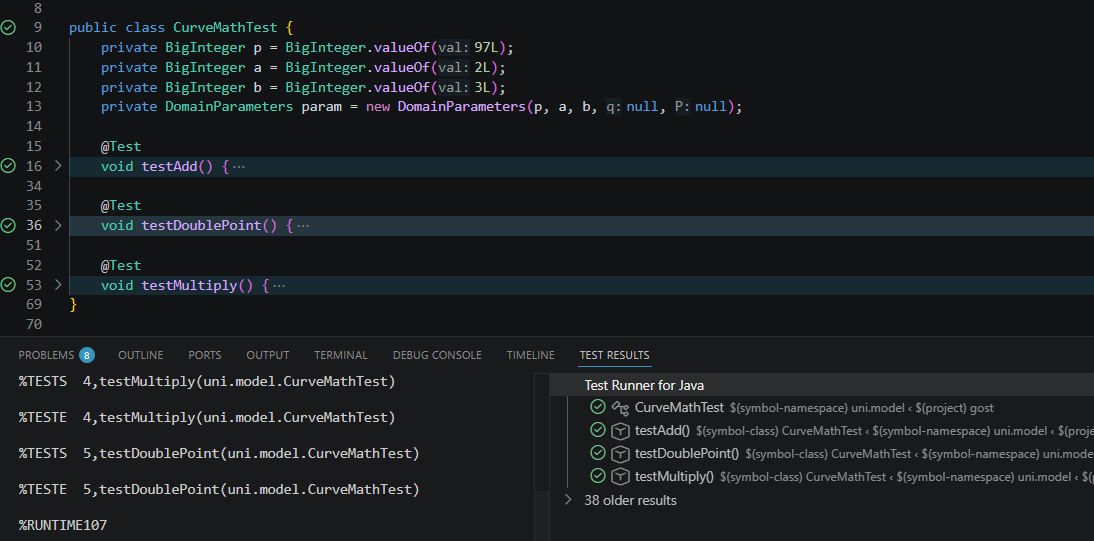
\includegraphics[width=0.85\textwidth]{imagenes/test_curvemath.png}
    \caption{Suite de pruebas unitarias ejecutadas con éxito para CurveMath.}
    \label{fig:test_curvemath}
\end{figure}

\subsection{Resultados de la Función Hash (\texttt{StreebogTest})}
Se procesaron cadenas de texto vacías, patrones repetitivos e instrucciones de prueba de la RFC 6986, validando las matrices de sustitución no lineal (\textit{S-Box}) y las transformaciones lineales de mezcla de bytes del algoritmo Streebog.

\begin{figure}[H]
    \centering
    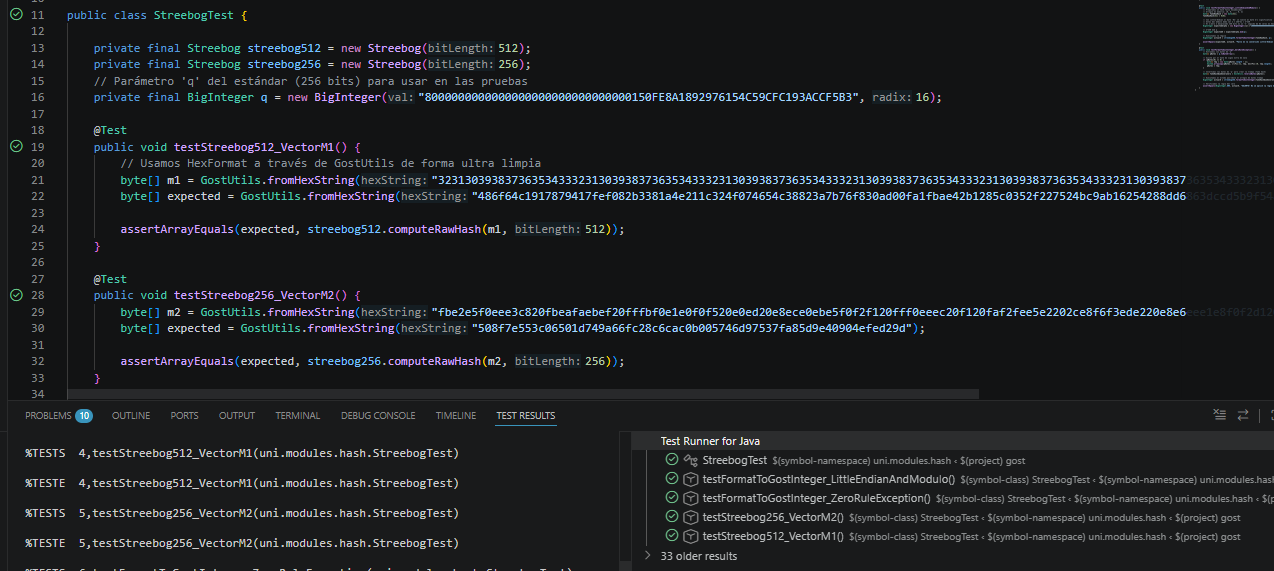
\includegraphics[width=0.85\textwidth]{imagenes/test_streebog.png}
    \caption{Verificación exitosa del vector de hash de 512 bits frente al estándar GOST R 34.11-2012.}
    \label{fig:test_streebog}
\end{figure}

\subsection{Resultados del Módulo Emisor (\texttt{SignatureGeneratorTest})}
Esta fase inyecta vectores pseudoaleatorios deterministicos para constatar que el cálculo de los componentes intermedios de la firma digital $(r, s)$ se adhiera a las especificaciones matemáticas del estándar ruso.

\begin{figure}[H]
    \centering
    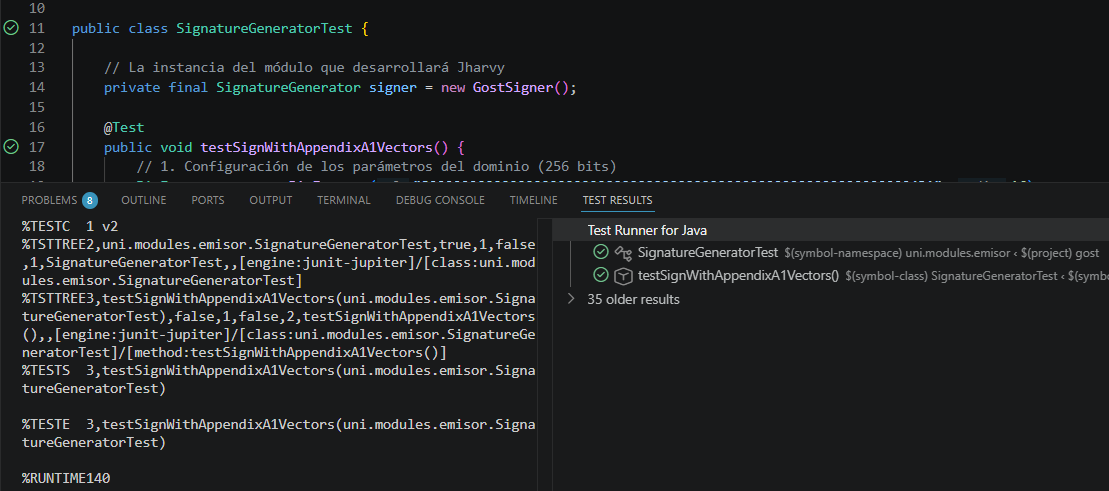
\includegraphics[width=0.85\textwidth]{imagenes/test_generator.png}
    \caption{Suite de aserciones de JUnit 5 validadas satisfactoriamente para GostSigner.}
    \label{fig:test_generator}
\end{figure}

\subsection{Resultados del Módulo Receptor (\texttt{SignatureVerifierTest})}
Las pruebas de este módulo aseguran la correcta validación de firmas auténticas y el rechazo estricto de firmas alteradas. Se verifica que la ecuación de validación reconstruya el componente $r$ original y se corrobora el manejo de casos borde, como el rechazo inmediato si los parámetros $r$ o $s$ se encuentran fuera del rango permitido ($0 < r, s < q$).

\begin{figure}[H]
    \centering
    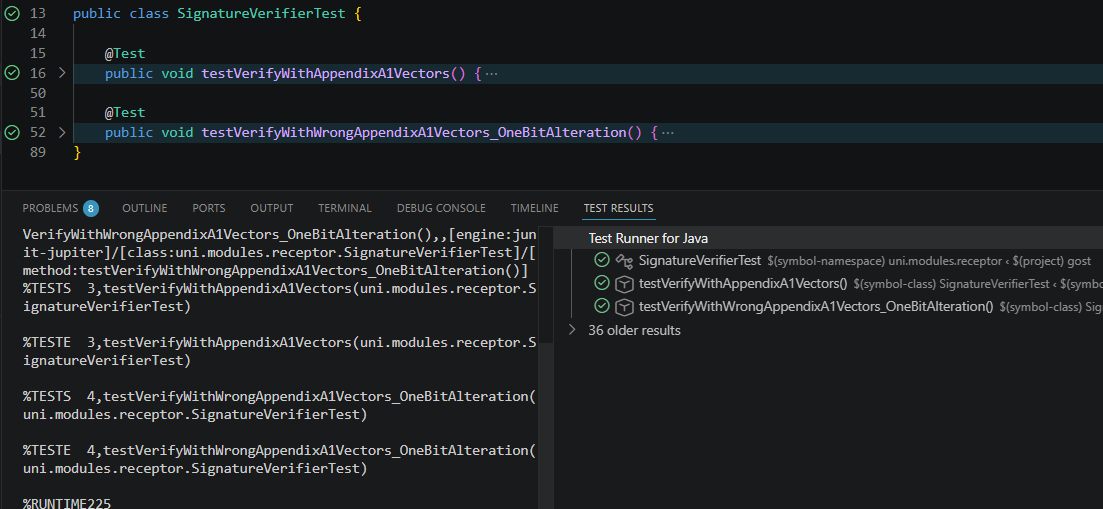
\includegraphics[width=0.85\textwidth]{imagenes/test_verifier.png}
    \caption{Resultados exitosos de las aserciones de validación de firma para GostVerifier.}
    \label{fig:test_verifier}
\end{figure}

\subsection{Log de Consola de la Aplicación Integrada}
Al compilar y ejecutar el proyecto utilizando el ciclo de vida de Maven, se genera la siguiente salida por consola, evidenciando el ciclo completo y exitoso de orquestación criptográfica:

\begin{figure}[H]
    \centering
    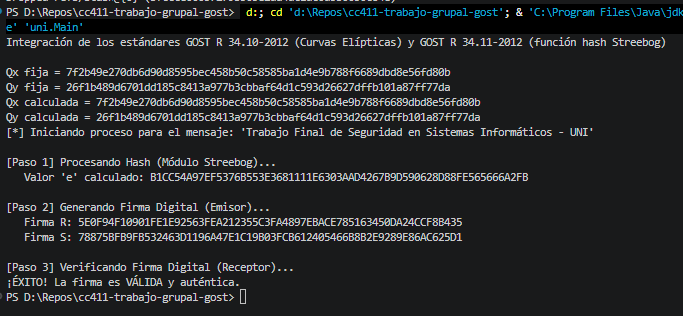
\includegraphics[width=0.85\textwidth]{imagenes/console_log.png}
    \caption{Captura de la salida estándar del sistema orquestador ejecutado en el entorno local.}
    \label{fig:console_log}
\end{figure}

\end{document}